\section{Résolution d'équations différentielles ordinaires}
Dans cette partie, on cherche à programmer différentes méthodes de résolution
des équations différentielles.
Ces algorithmes sont tous des méthodes à un pas, de la forme suivante :
	$y_{n+1}=y_n+h_n\phi (y_n,t_n,h_n)$ .

\subsection{Représentation d'un problème de Cauchy}
Tout d'abord, on cherche à définir la façon dont on va représenter
un problème de Cauchy dans notre code. Un problème de Cauchy est défini par :
\begin{equation}
    \begin{cases}
        y(t_0)=y_0 ~\text{Condition initiale}\\
        y’(t)=f(y(t),t)~\text{Equation différentielle} \\
    \end{cases}    
\end{equation}
On a donc décidé de définir $y_{0}$ comme étant une liste (numpy) de n éléments si la dimension est n. 
Pour y'(t), on a considéré que
c'était une fonction de y et t qui renvoie une liste (numpy) de n éléments si la dimension est n.
\subsection{Méthodes de résolution}
Ensuite, on a cherché à programmer les méthodes de résolution suivantes : méthode d’Euler, méthode du point milieu,
méthode de Heun et méthode de Runge-Kutta d’ordre 4. Elles correspondent respectivement aux équations
\ref{eq:euler}, \ref{eq:pointmilieu}, \ref{eq:heun} et \ref{eq:runge kutta}.
\begin{equation}
    y_{n+1} = y_n + h_n F (t_n, y(t_n))
    \label{eq:euler}
\end{equation}
\begin{equation}
    y_{n+1} = y_n + h_n  F(t_n + h_{\frac{n}{2}}, y_{n+ \frac{1}{2} })
    \label{eq:pointmilieu}
\end{equation}
\begin{equation}
        y_{n+1} = y_n + h_n \frac{F(t_n, y_n) + F(t_n+h_n, y_n + h_n F(t_n, y_n))}{2}
    \label{eq:heun}
\end{equation}
\begin{equation}
    \begin{cases}
        p_{n2} = F(t_n+\frac{1}{2}h_n,y_n+\frac{1}{2}h_n F(t_n, y_n))\\
        p_{n3} = F(t_n+\frac{1}{2}h_n,y_n+\frac{1}{2}h_n p_{n2})\\
        p_{n4} = F(t_n+h_n,y_n+h_n p_{n3})\\
        y_{n+1} = y_n + \frac{1}{6} h_n (F(t_n, y_n) + 2p_{n2} + 2p_{n3} + p_{n4})
    \end{cases}
    \label{eq:runge kutta}
\end{equation}

On a donc implémenté ces méthodes de la façon la plus générique possible. Tout d'abord, 
chaque fonction correspondant à une méthode est nommée sous la forme : step\_$<$name$>$(y,t,h,f) et calcule 
un seul pas de la méthode. Nous avons ensuite implémenté meth\_n\_step qui calcule un nombre N de pas de taille constante h,
puis meth\_epsilon qui calcule une solution approchée avec un paramètre d’erreur epsilon.
Nous avons aussi implémenté une fonction meth\_epsilon\_convergence qui nous a permis de voir
la convergence de nos solutions. Sur la Figure \ref{fig:subdivision}, on peut voir une comparaison
des convergences d'une fonction avec la méthode d'Euler. Comme attendu, on peut voir
que plus est N est grand plus ça converge vers la fonction initiale.

\begin{figure}[htbp!]
	\centering
	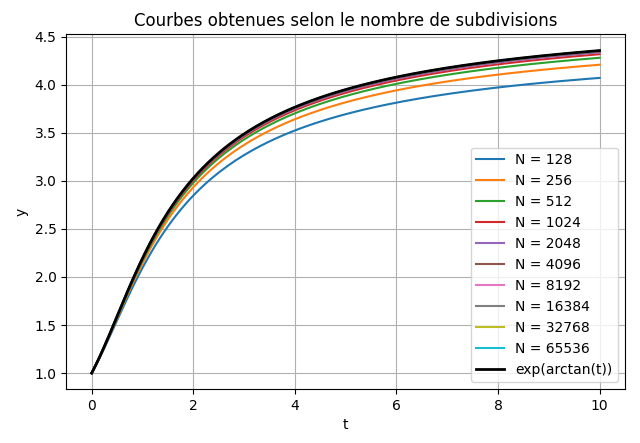
\includegraphics[width=0.5\textwidth]{res/subdivisions}
	\caption{Courbes comparant la convergence des solutions proposées par la méthode d'Euler en fonction du pas N}
	\label{fig:subdivision}
\end{figure}

L'implémentation générique des fonctions a permis d'avoir des résultats plus
précis même si ces résultats demandent un temps de calcul plus long pour des fonctions
plus complexes.\\
\subsection{Champ des tangentes}
Ensuite, nous avons implémenté la fonction tangent\_2D qui nous a permis de tracer le champ des tangentes
des équations différentielles de dimension 2. Comme on peut le voir sur la Figure
\ref{fig:tangente}, nous avons tracé cette courbe des tangentes sur un exemple d'équation différentielle
de dimension 2 de la forme $y(t)=(y_1(t),y_2(t))$ avec $y(0)=(1,0)$ et $y'(t)=(-y_2(t),y_1(t))$. Les résultats que nous
obtenons pour ces champs de tangentes sont proches des résultats exacts.

\begin{figure}[htbp!]
	\centering
	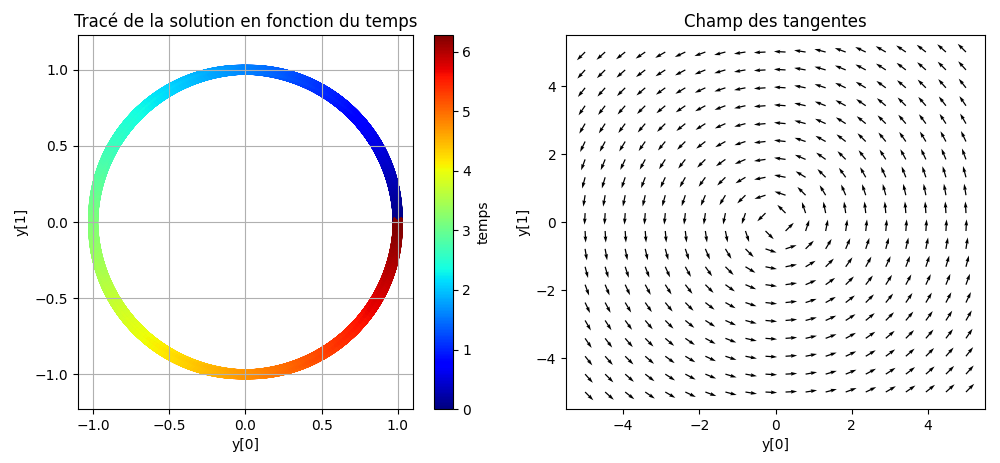
\includegraphics[width=0.7\textwidth]{res/tangente}
	\caption{Figures représentant le tracé de la solution de l'équation différentielle en fonction du temps et son champ des tangentes}
	\label{fig:tangente}
\end{figure}